
\begin{figure}
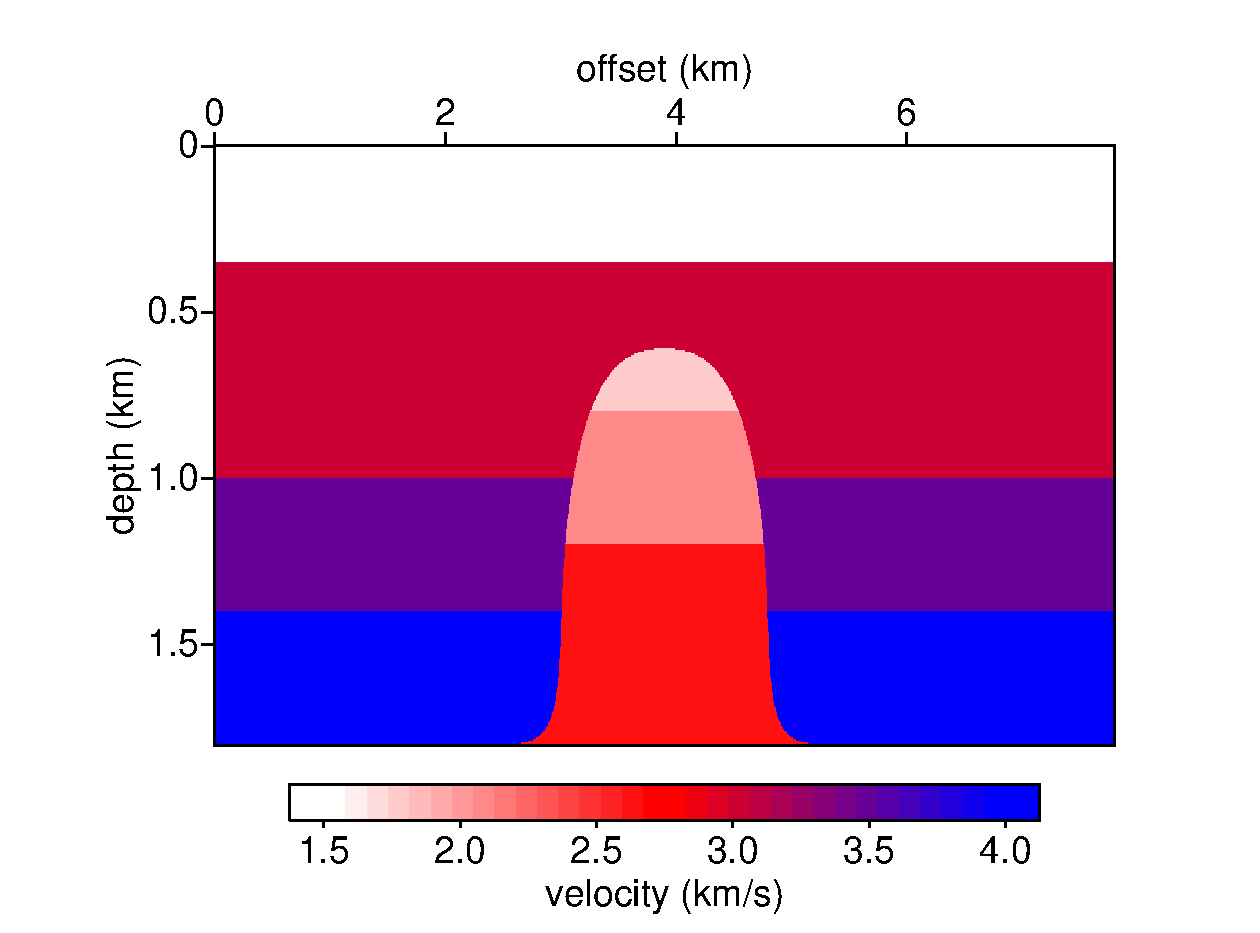
\includegraphics[height=10cm,width=15cm]{./Fig/fig1.ps}
\caption{Dome velocity model}
\label{fig:vp}
\end{figure}

\begin{figure}
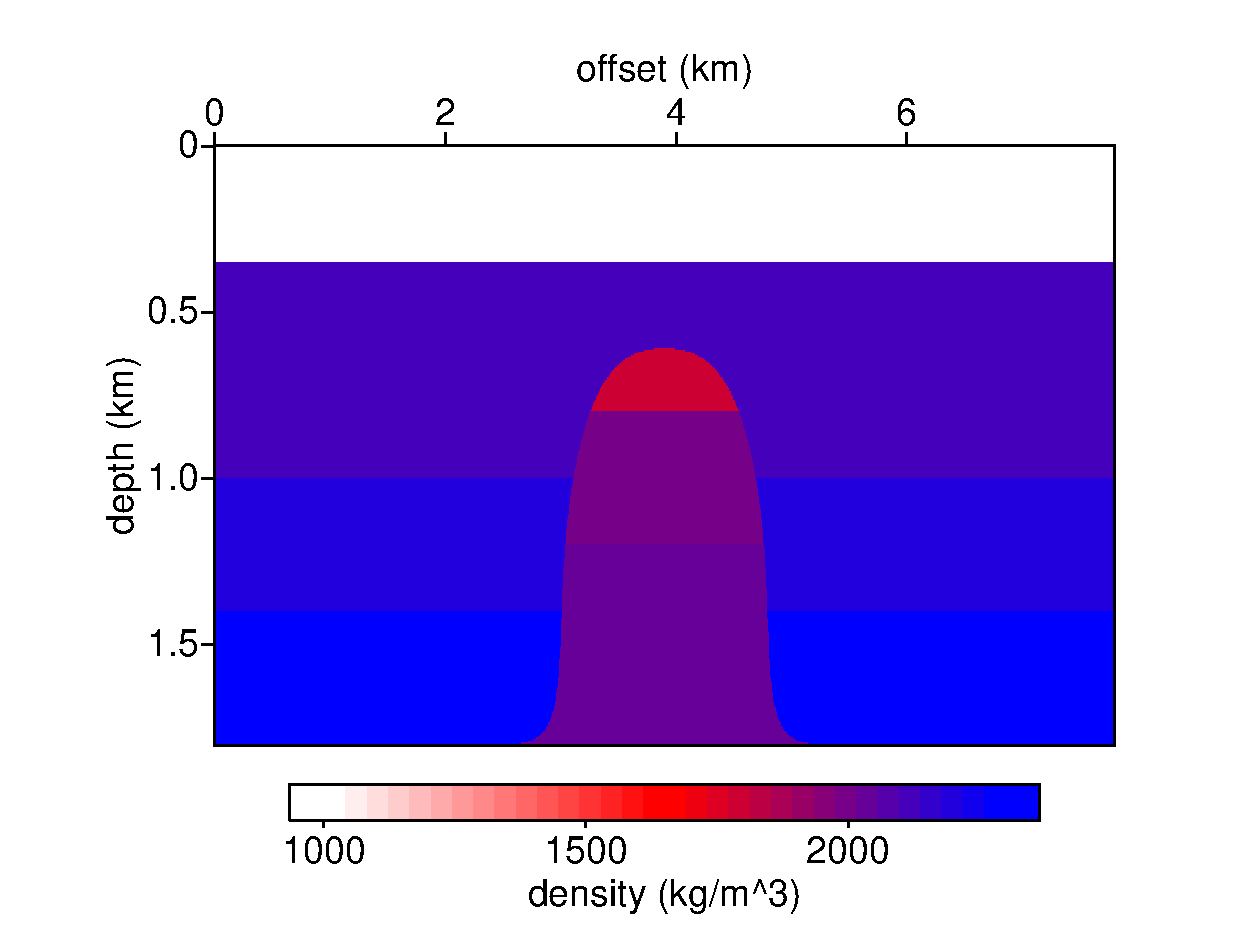
\includegraphics[height=10cm,width=15cm]{./Fig/fig2.ps}
\caption{Dome density model}
\label{fig:dn}
\end{figure}

\begin{figure}
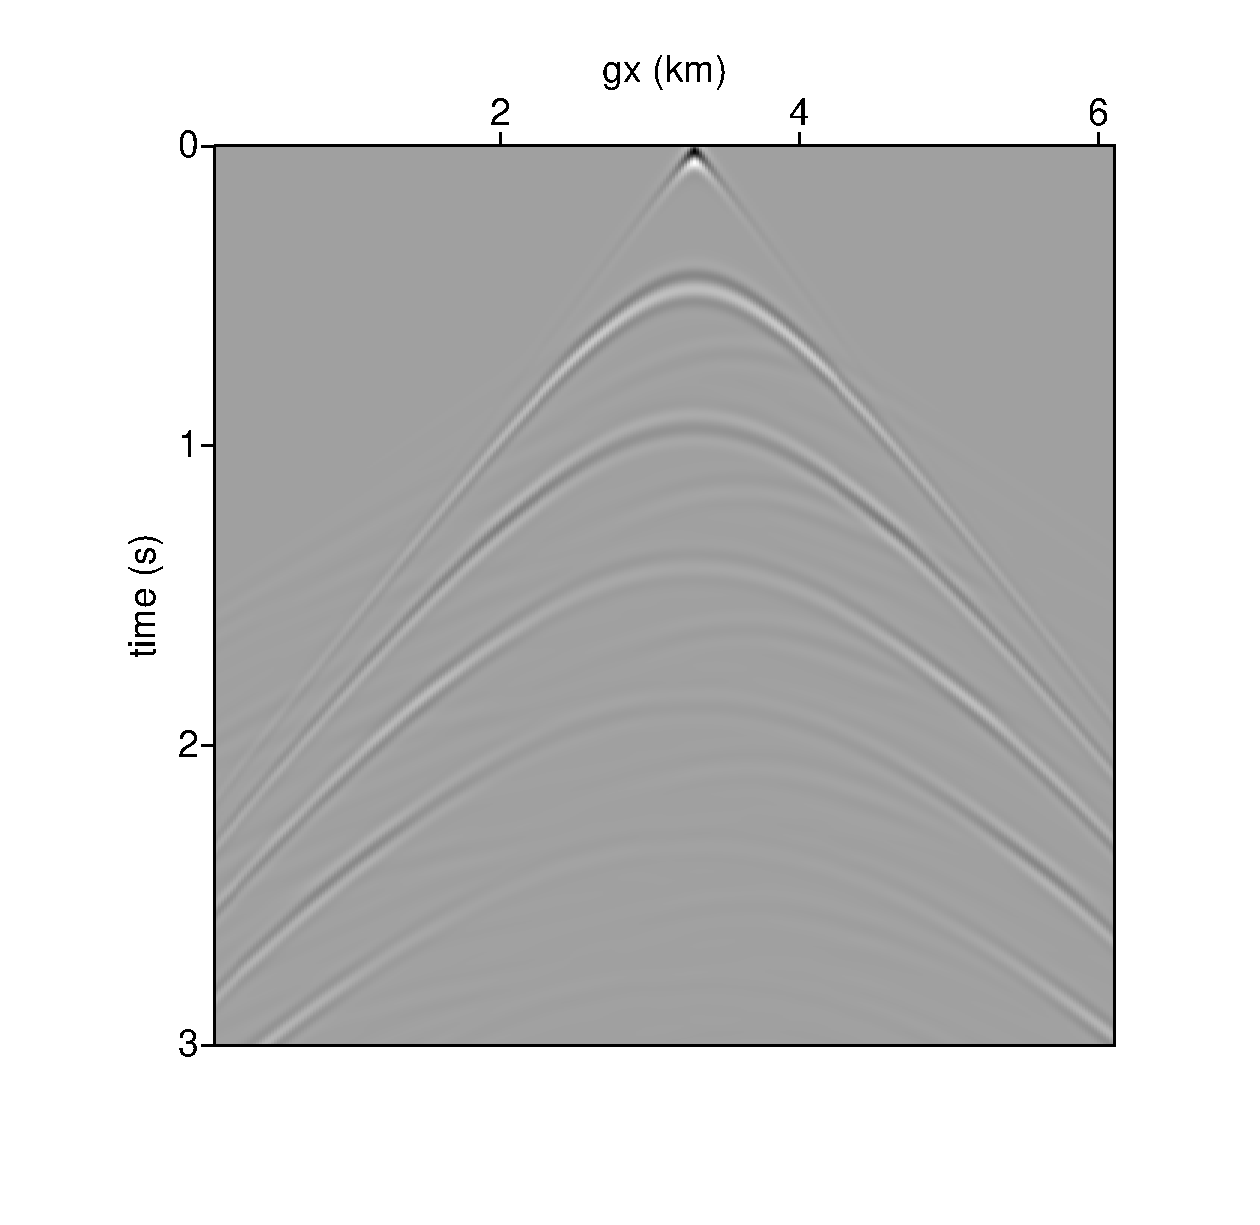
\includegraphics[height=15cm,width=15cm]{./Fig/fig3.ps}
\caption{2D shot record, (2,4) staggered grid scheme, $\Delta x = \Delta z =$ 5 m,
  appropriate $\Delta t$, 301 traces: shot x = 3300 m, shot z = 40 m, receiver x =
 100 - 6100 m, receiver z = 20 m, number of time samples = 1501, time
sample interval = 2 ms. Isotropic point source, pulse = Ricker wavelet, 10 Hz center frequency.}
\label{fig:data5m}
\end{figure}

\begin{figure}
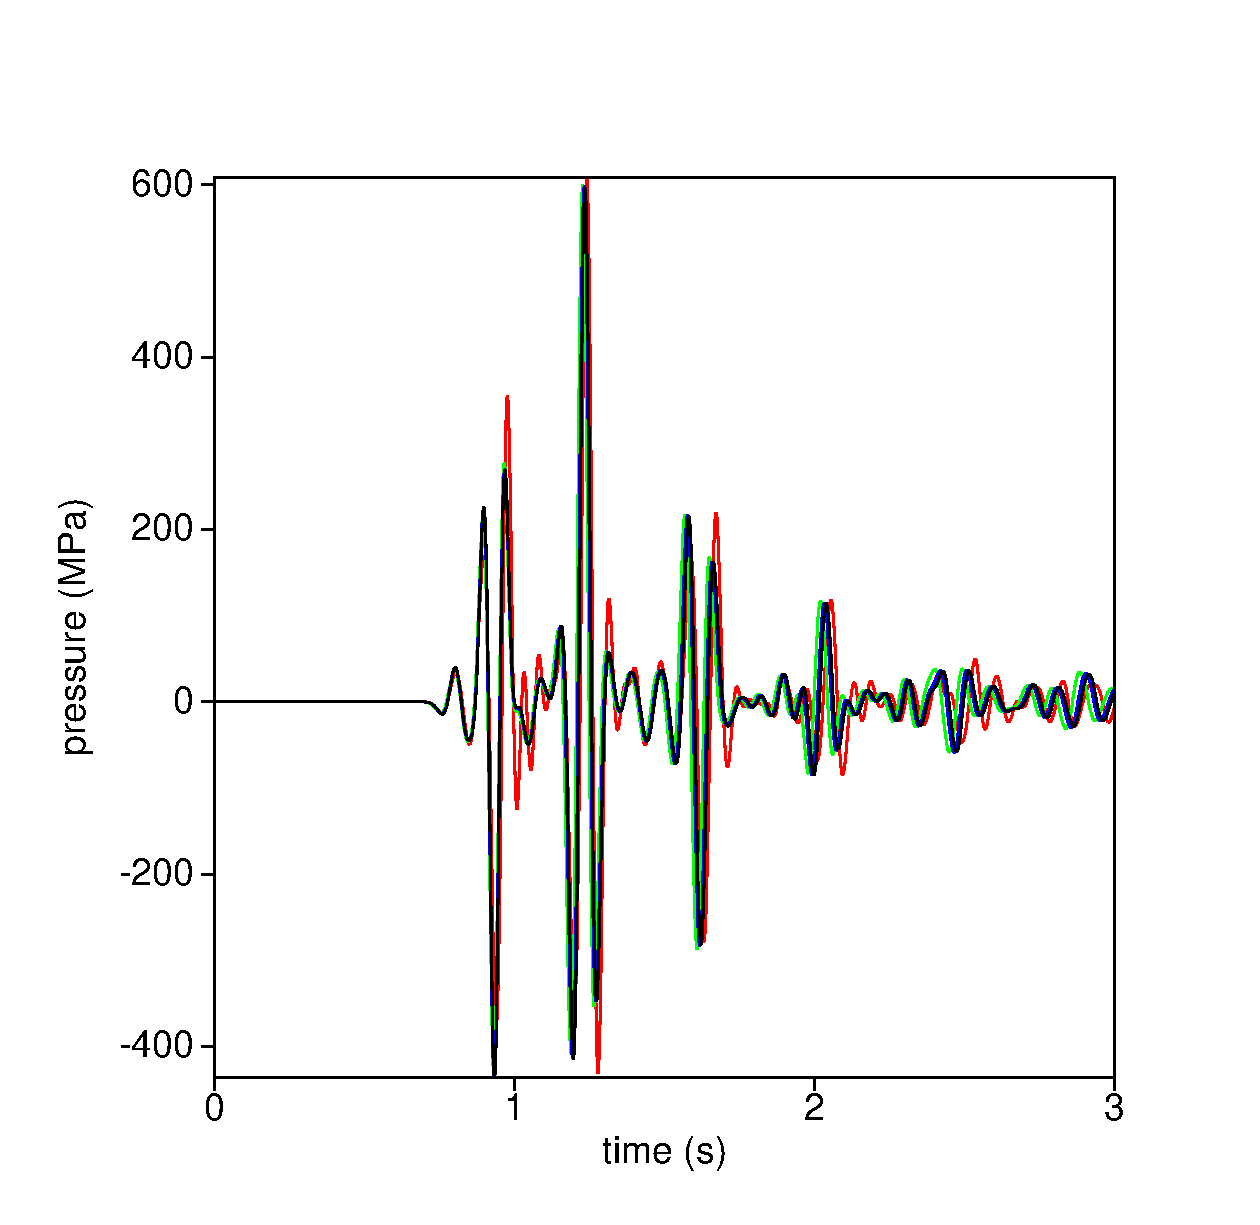
\includegraphics[height=15cm,width=15cm]{./Fig/fig4.ps}
\caption{Trace 100 (receiver x = 2100 m) for $\Delta x = \Delta z = $
  20 m (red), 10 m (green), 5 m (blue), and 2.5 m (black). Note
  arrival time discrepancy after 1 s: this is the interface error
  discussed in \cite{SymesVdovina:09}. Except for the 20 m result,
  grid dispersion error is minimal.} 
\label{fig:trace}
\end{figure}

\begin{figure}
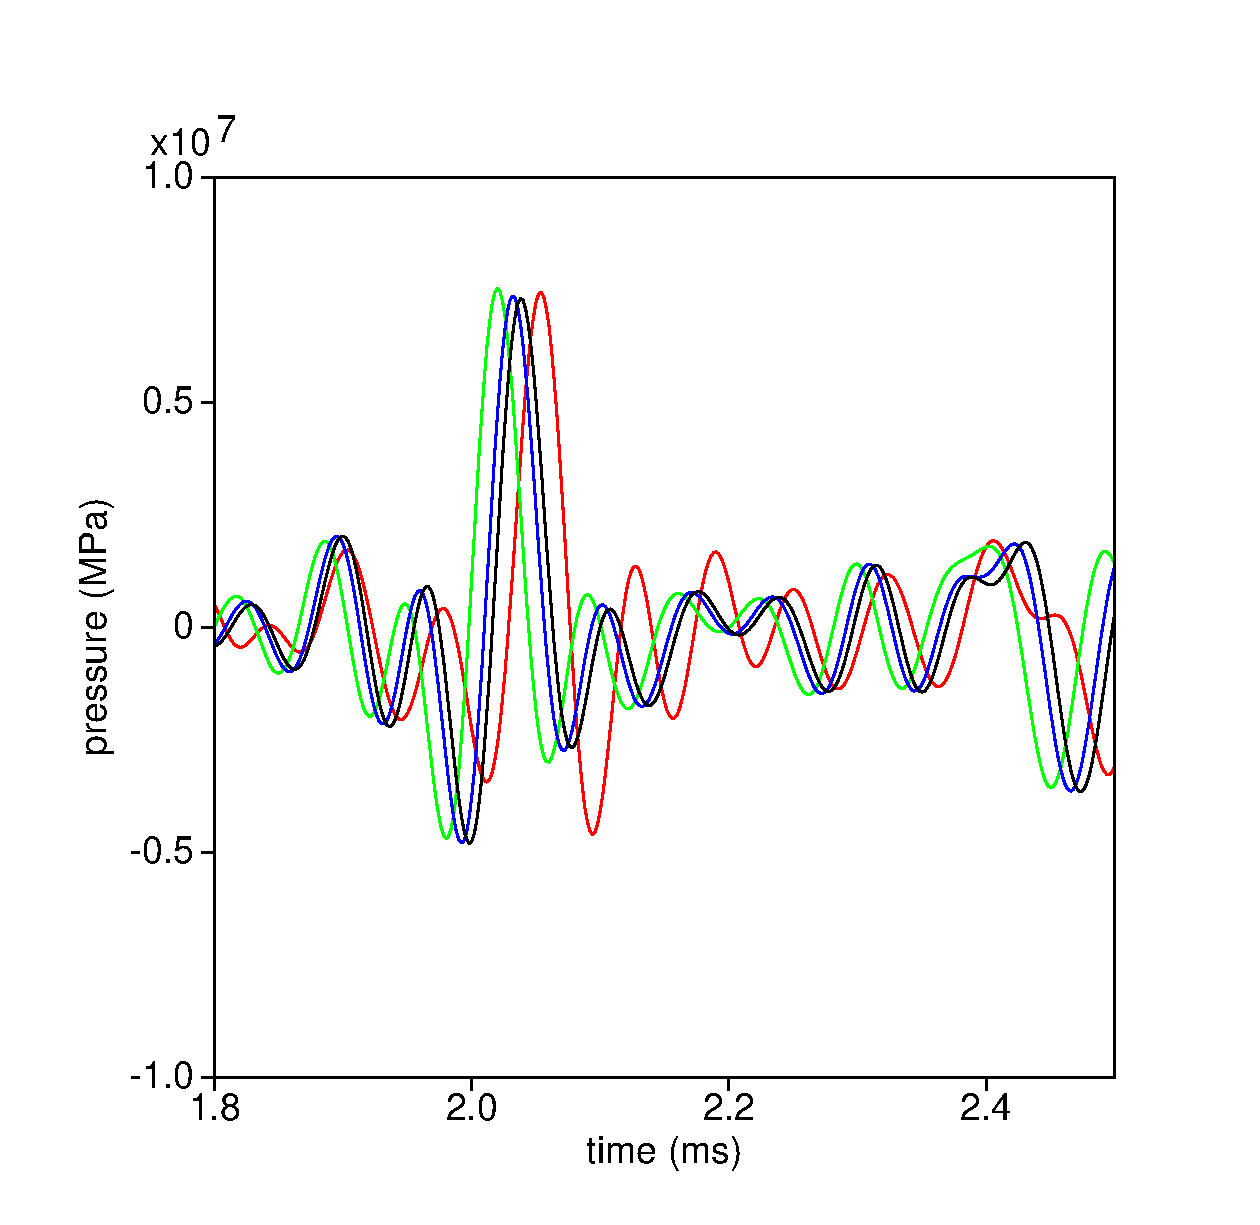
\includegraphics[height=15cm,width=15cm]{./Fig/fig5.ps}
\caption{Trace 100 detail, 1.8-2.5 s, showing more clearly the
  first-order interface error: the time shift between computed events
  and the truth (the 2.5 m result, more or less) is proportional to
  $\Delta t$, or equivalently to $\Delta z$.}
\label{fig:wtrace}
\end{figure}

\begin{figure}
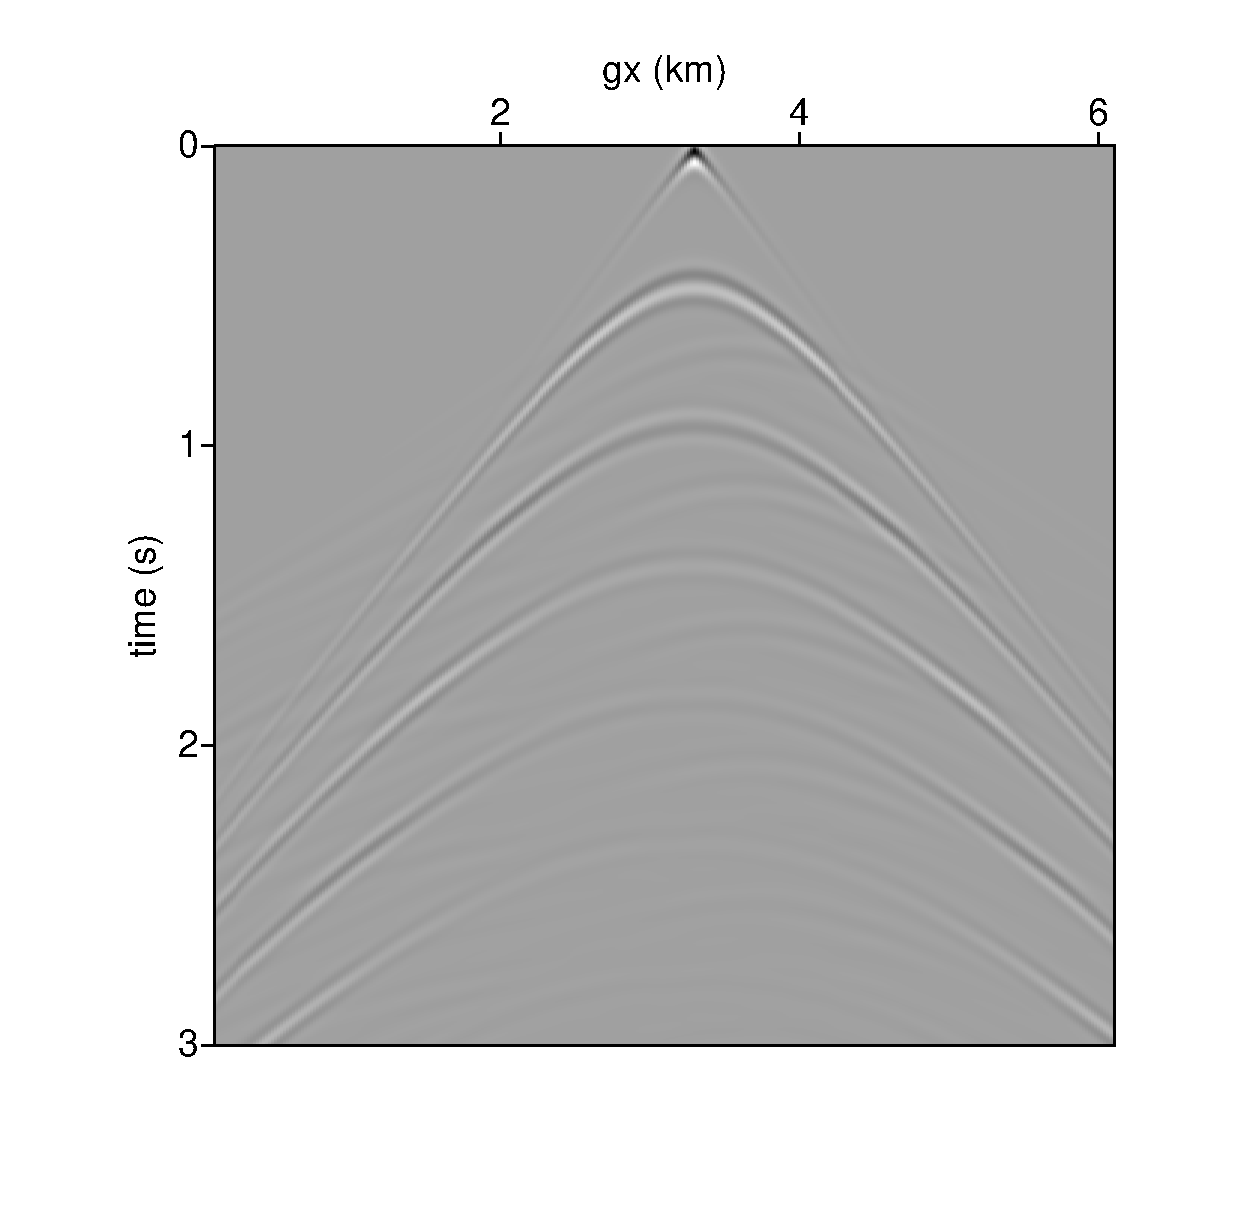
\includegraphics[height=15cm,width=15cm]{./Fig/fig6.ps}
\caption{2D shot record, (2,8) scheme, other
  parameters as in Figure \ref{fig:data5m}.}
\label{fig:data5m8k}
\end{figure}

\begin{figure}
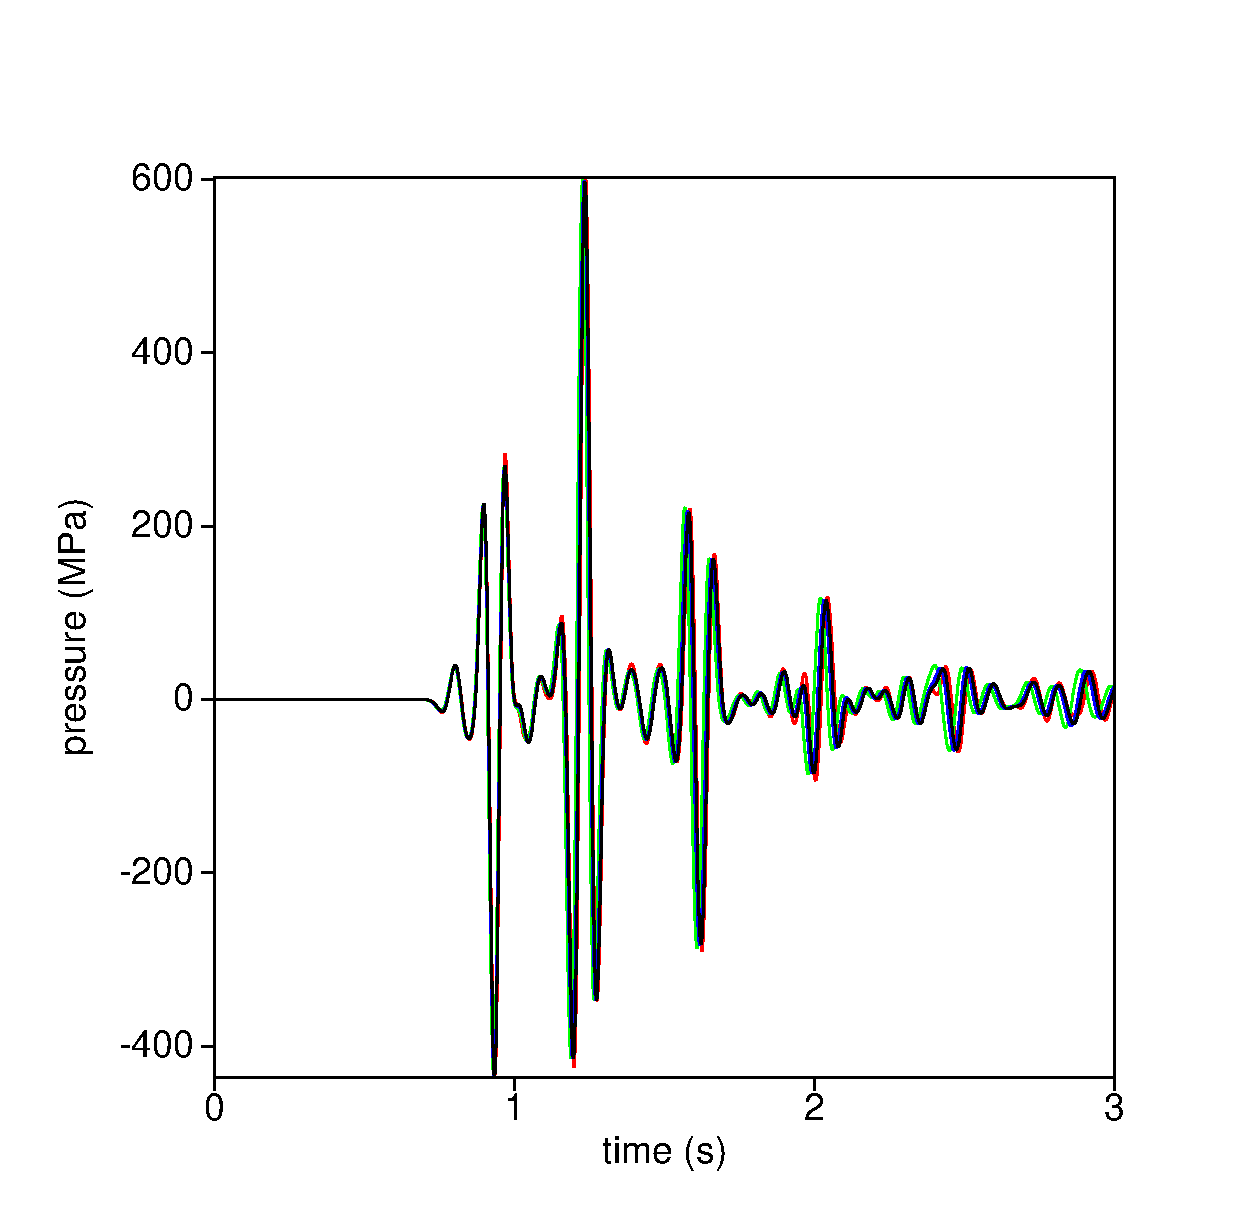
\includegraphics[height=15cm,width=15cm]{./Fig/fig7.ps}
\caption{Trace 100 computed with the (2,8) scheme,
  other parameters as described in the captions of Figures
  \ref{fig:data5m} and \ref{fig:trace}.} 
\label{fig:trace8k}
\end{figure}

\begin{figure}
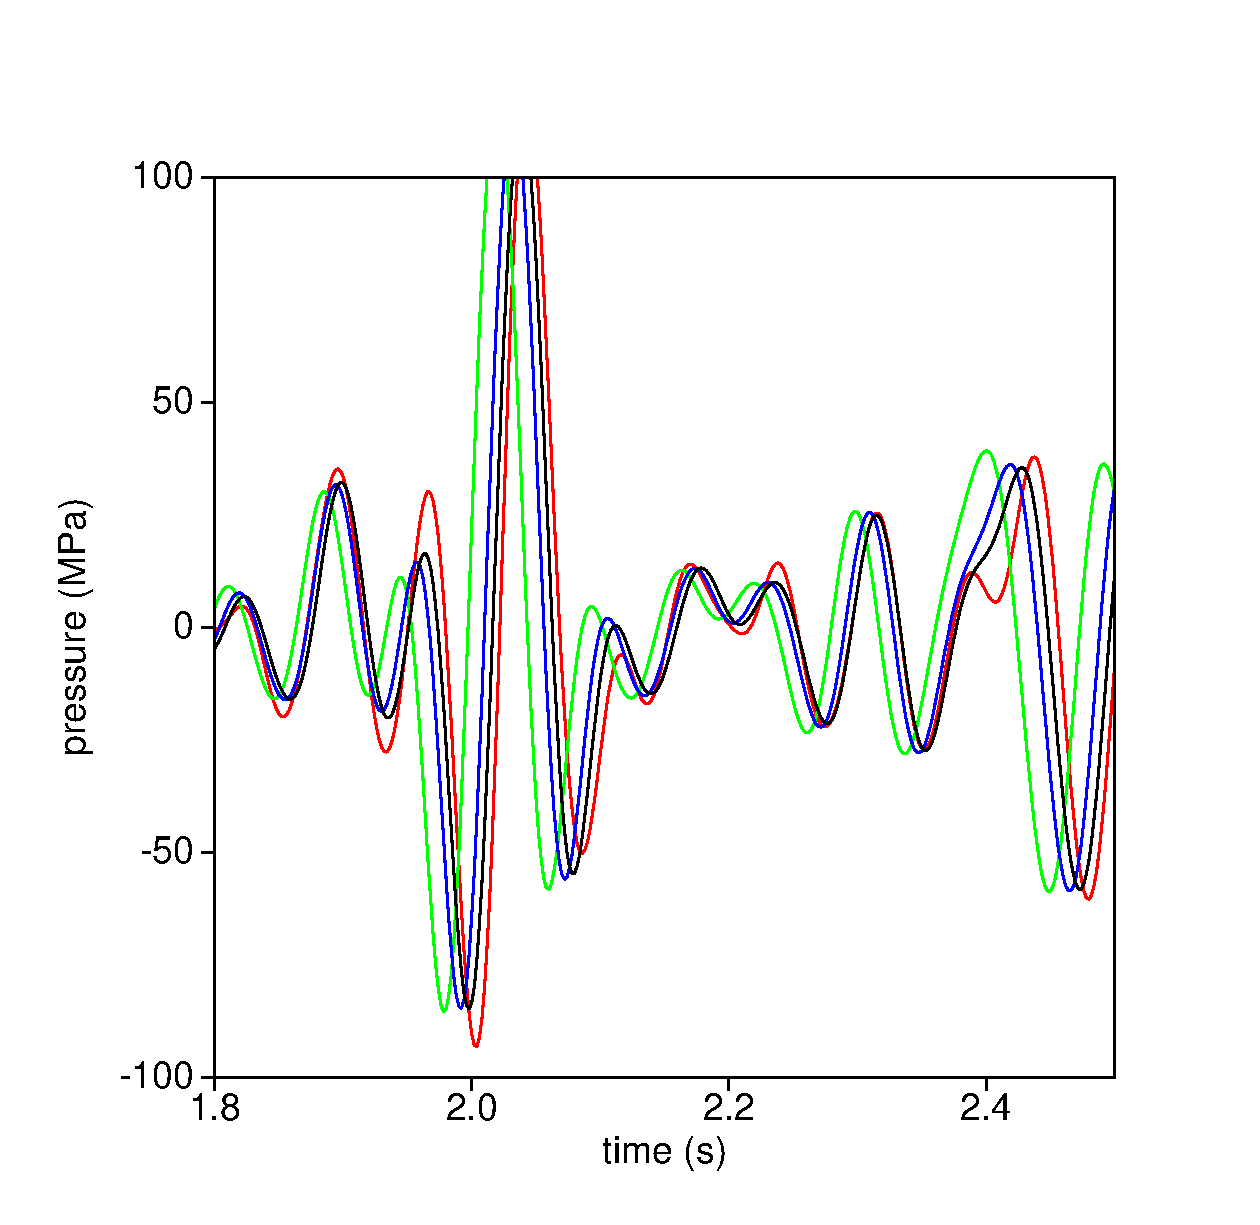
\includegraphics[height=15cm,width=15cm]{./Fig/fig8.ps}
\caption{Trace 100 detail, 1.8-2.5 s, (2,8) scheme..
Comparing to Figure \ref{fig:wtrace}, notice that the dispersion error for
the 20 m grid is considerably smaller, but the results for finer grids
are nearly identical to those produced by the (2,4) grids - almost all
of the remaining error is due to the presence of discontinuities in
the model.}
\label{fig:wtrace8k}
\end{figure}